\documentclass[a4paper]{article}
\title{Assignment 1}
\author{Student: Harkeerat Singh Sawhney\\Student's email: sawhnh@usi.ch } %%%%%%%%%%%% Modify here!!!!
\date{}

%%%%%%%%%%%%%%%%%%%
% Packages
%%%%%%%%%%%%%%%%%%
\usepackage{amsmath}
\usepackage{bm}
\usepackage{hyperref}
\usepackage{verbatim}
\usepackage{graphicx}
\usepackage{enumerate}
\usepackage{xcolor}
\usepackage{listings}
\usepackage{listings}
\usepackage{xcolor}
\usepackage{float}
\usepackage{amsmath}
\usepackage{amsmath, amssymb} % for math symbols and fonts
\usepackage{hyperref} % for hyperlinks
\usepackage{listings}
\usepackage{xcolor}
\usepackage{subcaption}



\lstdefinestyle{mystyle}{
    language=Python,
    basicstyle=\ttfamily,
    keywordstyle=\color{blue},
    commentstyle=\color{green!50!black},
    stringstyle=\color{orange},
    numbers=left,
    numberstyle=\tiny,
    numbersep=5pt,
    backgroundcolor=\color{gray!5},
    frame=single,
    showspaces=false,
    showstringspaces=false,
    showtabs=false,
    tabsize=4,
    breaklines=true,
    breakatwhitespace=true,
}







%%%%%%%%%%%%%%%%%%%	
% Commands
%%%%%%%%%%%%%%%%%%
\newcommand{\erre}{\mathbf{R}}
\newcommand{\link}[2]{\href{#1}{\textcolor{blue}{#2}}}


\begin{document}
\maketitle

\section*{Polynomial regression}
Write answers to questions here. Please, keep the original enumeration.

\begin{enumerate}
	\item In Question 1 it was asked to implement a function PlotPolynomial, which plots the function $ p(z) = \sum_{k=1}^{4} z^k w_k $. The function took \textit{coeffs} which is a \texttt{np.array} and contains the 5 weights $ w_{0}, w_{1}, w_{2}, w_{3}, w_{4} $. In that $ w_{0} = 0 $. The function also took a z-range which is the range for the z value. The function then plots the polynomial function $ p(z) $ for the given z-range. This was done by the use of the python library \texttt{matplotlib.pyplot}. To test the function out the following variable were used.


	      \begin{lstlisting}[style=mystyle]
coeffs = np.array([0, -10, 1, -1, 1 / 1000])
z_range = [-10, 10]
color = "b"
plot_polynomial(coeffs, z_range, color)
\end{lstlisting}

	      The figure generate from the function can be seen in Figure \ref{fig:question1}.
	      \begin{figure}[H]
		      \centering
		      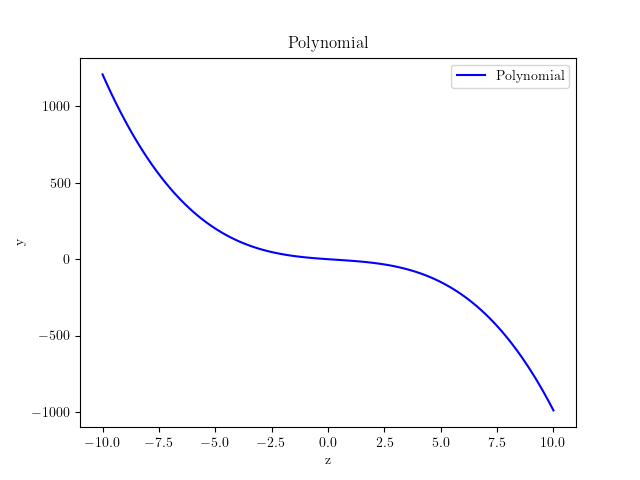
\includegraphics[width=0.8\textwidth]{../Graph/polynomial-question1.png}
		      \caption{Polynomial function generated from the function \texttt{plot\_polynomial}}
		      \label{fig:question1}
	      \end{figure}

	\item In Question 2 we were asked to make a function \texttt{createDataset}, which is similar to the function \texttt{createDataset} from the previous assignment. The function take the following parameters, \texttt{coeffs} which is a \texttt{np.array} containing the weights $ w_{0}, w_{1}, w_{2}, w_{3}, w_{4} $, \texttt{z\_range} which is the range of the z values, \texttt{N} which is the number of samples to be generated, \texttt{sigma} which is the standard deviation of the noise and \texttt{seed} which is the seed for the random number generator.

	      First a random state is initialized with the seed provided, then through zMin and zMax the set of sampleSize z values are generated. Lastly through the definition of the $ D` $ dataset the x values are computed for the power of 0 to 4. Hence at last x is a matrix of size $ sampleSize \times 5 $.

	      After that the value of y had to be computed using the formula $ y = xw + \epsilon $, where $ \epsilon $ is the noise. This was done by first generating a noise vector of size $ SampleSize \times 1 $ and then adding it to the xw vector. The noise vector was generated using the \texttt{randn} function from the \texttt{numpy.random} library. The function at last returns the x and y values.

	      The function starts from line 54.

	\item In Question 3 we were given the values of the parameters for the function \texttt{createDataset} and were asked to generate the dataset. We were asked to generate 2 dataset, one for the training and one for the testing. The training dataset was generated using the following parameters.

	      \begin{lstlisting}[style=mystyle]
coeffs = np.array([0, -10, 1, -1, 1 / 1000])
z_range = [-3, 3]
sigma = 0.5
sample_size_train = 500
sample_size_eval = 500
seed_train = 0
seed_eval = 1

# Creating the dataset
X_train, y_train = create_dataset(coeffs, z_range, sample_size_train, sigma, seed_train)
X_eval, y_eval = create_dataset(coeffs, z_range, sample_size_eval, sigma,seed_eval)

\end{lstlisting}



	\item In Question 4 we were asked to implement the function \texttt{visualizeDataset}. The function takes the x and y value which the function \texttt{createDataset} returns. The function then plots the x and y values using the \texttt{matplotlib.pyplot} library. The function also plots the polynomial function $ p(z) $ using the \texttt{plot\_polynomial} function.

	      \begin{figure}[H]
		      \centering
		      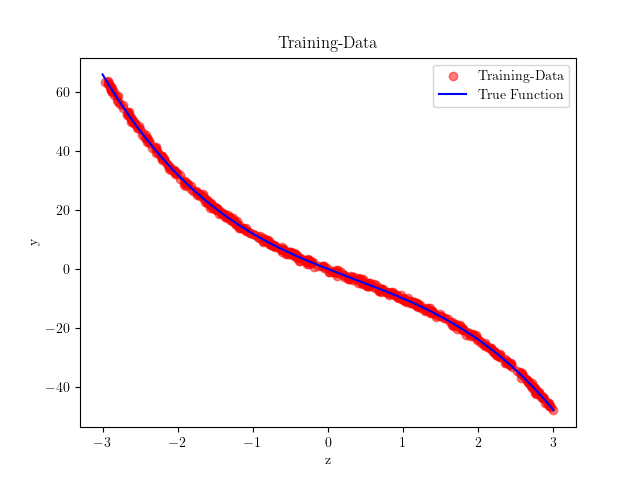
\includegraphics[width=0.8\textwidth]{../Graph/Training-Data.png}
		      \caption{Training Data vs True Polynomial}
		      \label{fig:question4a}
	      \end{figure}
	      Figure \ref{fig:question4a} shows the plot of the training data and the true polynomial function. As it can be seen from the plot that the data is not exactly on the True Polynomial function, because of the noise which is added to it.

	      \begin{figure}[H]
		      \centering
		      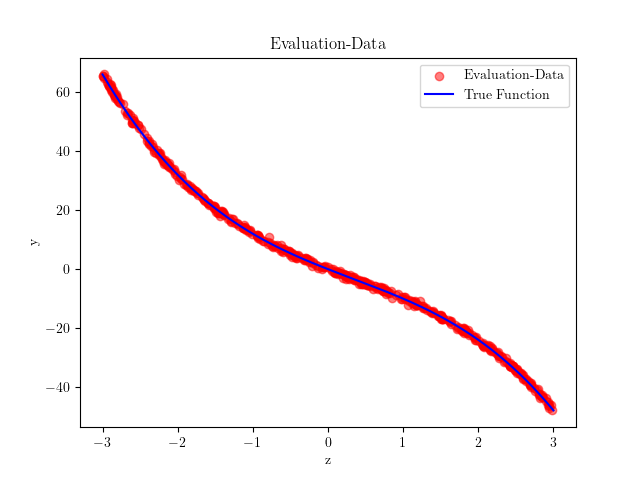
\includegraphics[width=0.8\textwidth]{../Graph/Evaluation-Data.png}
		      \caption{Evaluation Data vs True Polynomial}
		      \label{fig:question4b}
	      \end{figure}
	      Figure \ref{fig:question4b} shows the plot of the evaluation data and the true polynomial function. Again as it can be seen from the plot that the data is not exactly on the True Polynomial function, because of the noise which is added to it.
	\item In this Question we were asked to perform Polynomial Regression on the dataset $ D $. To achieve this there were in total 3 steps. First we had to preprocess the data, then we had to train the model and lastly we had to evaluate the model.

	      In order to preprocess the data we first need to reshape both training and evaluation data into the input and output dimensions. For the \texttt{X\_train} and \texttt{X\_eval} we need to reshape them into $ sampleSize \times 5 $ and for the \texttt{y\_train} and \texttt{y\_eval} we need to reshape them into $ sampleSize \times 1 $. The reason why for X we need to reshape it into $ sampleSize \times 5 $ is because we have 5 features (which are the weights) and for y we need to reshape it into $ sampleSize \times 1 $ because we have only 1 output. After that the data is converted into PyTorch tensors of type float32, and they were moved on the GPU for faster computation. With this data is ready to be trained on.

	      The second step is to prepare the model itself, and for this we created a class \texttt{PolynomialRegression}. The class inherits from the \texttt{nn.Module} class, since we want to make a basic neural network module. The neural network is very simple as it has only one layer which takes 5 inputs and gives out 1 input. In the one fully connect layer it performs Linear Regression on the data.

	      At last third step is to put train the model with the processed data. For this we first initialize the model and then we define the loss function and the optimizer. The loss function is the Mean Squared Error (MSE) and the optimizer is the Stochastic Gradient Descent (SGD). The model is then trained for 5000 epochs and the loss is printed after every 100 epochs. The learning rate which was used in this case is 0.001. In the for loop the model is trained on the training data, and then is evaluation on the evaluation data. The loss is calculated for both the training and the evaluation data.

	      Some observations which I had noticed was with regarding the learning rate. If the learning rate is very high, then the loss would go to infinity and would not come down, but in the other hand if the learning rate is very low, it would never get towards the minimum loss. Hence the learning rate has to be chosen very carefully. The learning rate which I had chosen was 0.001, and it gave me the best results. Also another thing which I noticed was that initially in my neural network I had multiple layers and many neurons. This was mainly due to my misunderstanding of the question, but what I had observed was that the learning rate had to be much smaller due to the increase in the size of the neural network. 

	      Bias term in \texttt{torch.nn.linear} is the first weight, and since the first weight in our case is always 0 we do not need to add the bias term. Hence the bias term in \texttt{torch.nn.linear} can be false.

	      The code for this question starts from line 98.

	\item In this Question we were asked to plot the training and evaluation loss as functions of the epoch number. The plot can be seen in Figure \ref{fig:question6}.

	      \begin{figure}[H]
		      \centering
		      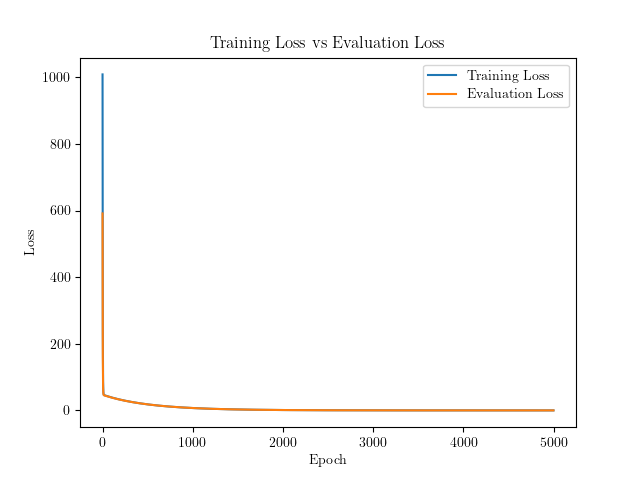
\includegraphics[width=0.8\textwidth]{../Graph/Training-Evaluation-Loss.png}
		      \caption{Training and Evaluation Loss vs Epochs}
		      \label{fig:question6}
	      \end{figure}
	      As it can be seen from the Figure \ref{fig:question6} that the training loss and evaluation loss is decreasing at the same rate and they are very close to each other. This means that the model is not overfitting and is generalizing well. However in the beginning the Training Loss is very high as compare to the Evaluation Loss, but in couple of epochs it comes down and then both the losses are very close to each other.
	\item In this Question we were asked to plot the polynomial from the true coefficients and the polynomial from the learned coefficients.

	      \begin{figure}[H]
		      \centering
		      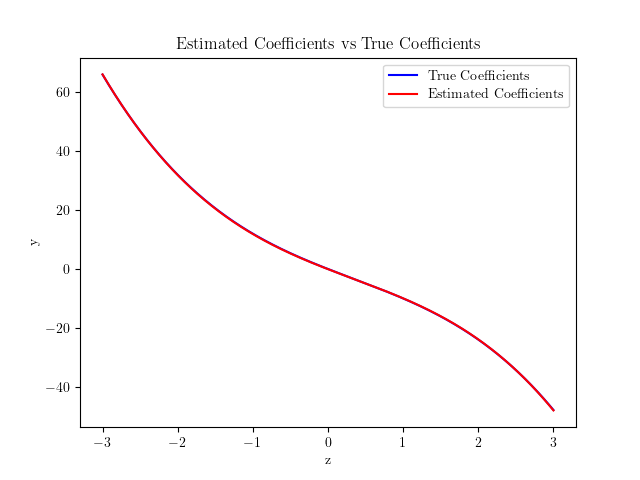
\includegraphics[width=0.8\textwidth]{../Graph/Estimated-True-Coefficients.png}
		      \caption{Estimated Coefficients vs True Coefficients}
		      \label{fig:question7}
	      \end{figure}
	      In the Figure \ref{fig:question7} we can see the plot of the estimated coefficients vs the true coefficients. As it can be seen from the plot that the estimated coefficients are very close to the true coefficients. This means that the model has learned the coefficients very well.
	\item Bellow are the 5 Figures showing the true weights vs the estimated weights per epoch.

	      \begin{figure}[H]
		      \centering
		      \begin{subfigure}{0.4\textwidth}
			      \centering
			      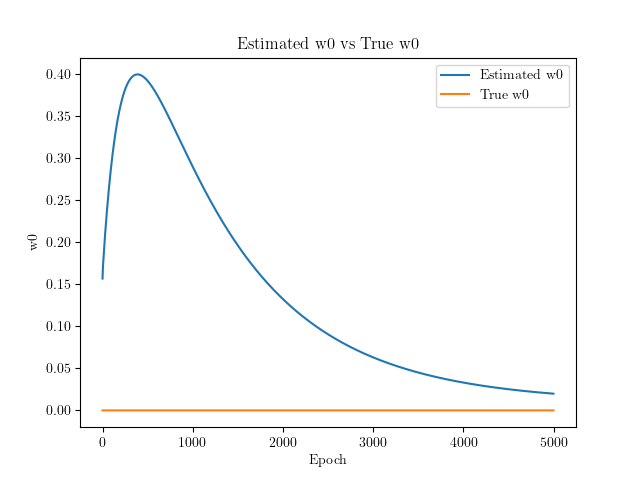
\includegraphics[width=\linewidth]{../Graph/Estimated-True-w0.png}
			      \caption{Estimated $w_0$ vs True $w_0$}
			      \label{fig:question8a}
		      \end{subfigure}
		      \hfill
		      \begin{subfigure}{0.4\textwidth}
			      \centering
			      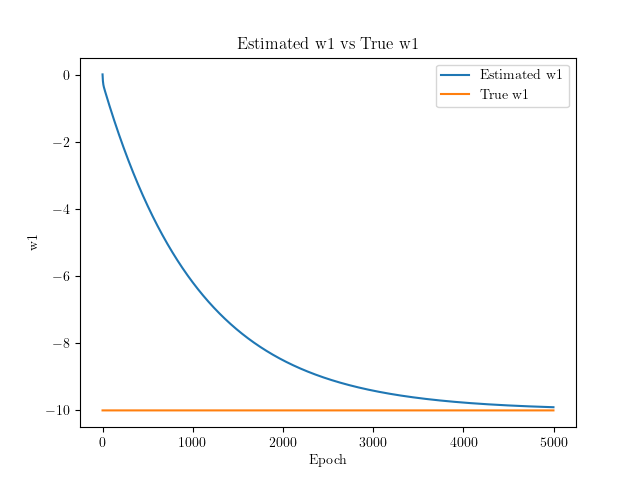
\includegraphics[width=\linewidth]{../Graph/Estimated-True-w1.png}
			      \caption{Estimated $w_1$ vs True $w_1$}
			      \label{fig:question8b}
		      \end{subfigure}

		      \begin{subfigure}{0.4\textwidth}
			      \centering
			      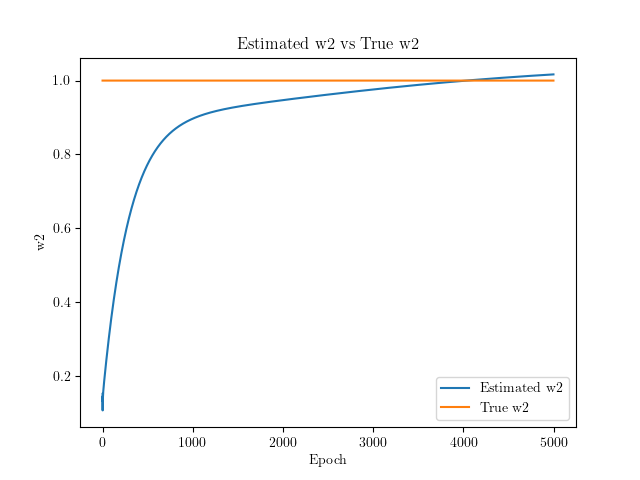
\includegraphics[width=\linewidth]{../Graph/Estimated-True-w2.png}
			      \caption{Estimated $w_2$ vs True $w_2$}
			      \label{fig:question8c}
		      \end{subfigure}
		      \hfill
		      \begin{subfigure}{0.4\textwidth}
			      \centering
			      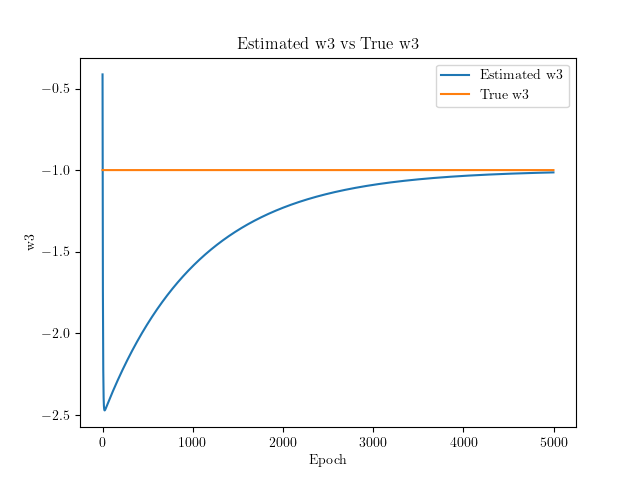
\includegraphics[width=\linewidth]{../Graph/Estimated-True-w3.png}
			      \caption{Estimated $w_3$ vs True $w_3$}
			      \label{fig:question8d}
		      \end{subfigure}

		      \begin{subfigure}{0.4\textwidth}
			      \centering
			      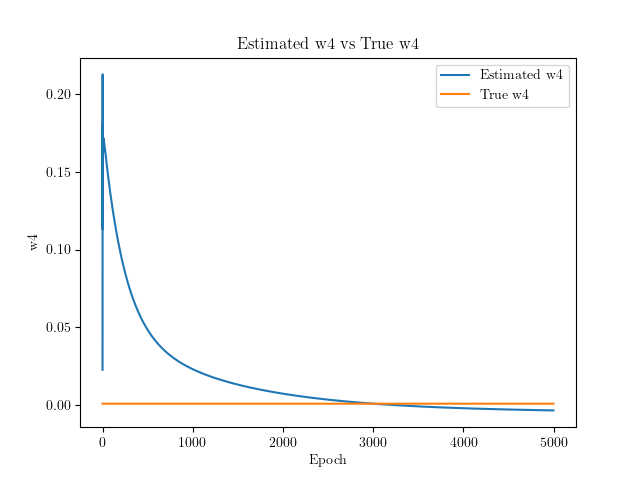
\includegraphics[width=\linewidth]{../Graph/Estimated-True-w4.png}
			      \caption{Estimated $w_4$ vs True $w_4$}
			      \label{fig:question8e}
		      \end{subfigure}
		      \caption{Comparison of Estimated and True $w$ values}
		      \label{fig:question8}
	      \end{figure}

	\item
	      As it can be seen from the Figure \ref{fig:question8} that the estimated weights are very close to the true weights. This means the model has been trained very well and has learned the weights very well.
	      \newpage

	      \begin{lstlisting}[style=mystyle]
coeffs = np.array([0, -10, 1, -1, 1 / 1000])
z_range = [-3, 3]
sigma = 0.5
sample_size_train = 10
sample_size_eval = 500
seed_train = 0
seed_eval = 1
# Creating the dataset
X_train, y_train = create_dataset(
coeffs, z_range, sample_size_train, sigma, seed_train
)
X_eval, y_eval = create_dataset(coeffs, z_range, sample_size_eval, sigma, seed_eval)

\end{lstlisting}

	      As it can be seen the main difference is the sample size of the training data. In the previous case the sample size was 500, but in this case the sample size is 10.

	      \begin{figure}[H]
		      \centering
		      \begin{minipage}{0.45\textwidth}
			      \centering
			      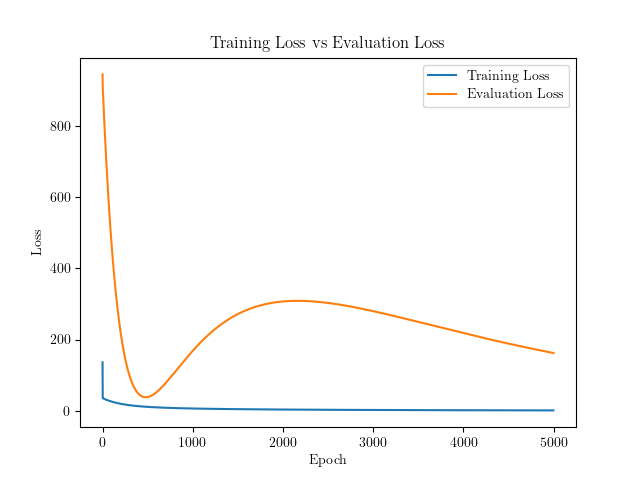
\includegraphics[width=\linewidth]{../Graph/Training-Evaluation-Loss2.png}
			      \caption{Training and Evaluation Loss vs Epochs}
			      \label{fig:question9a}
		      \end{minipage}
		      \hfill
		      \begin{minipage}{0.45\textwidth}
			      \centering
			      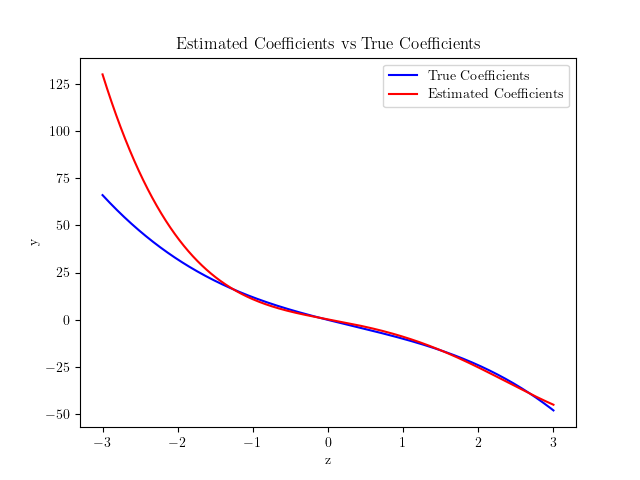
\includegraphics[width=\linewidth]{../Graph/Estimated-True-Coefficients2.png}
			      \caption{Estimated Coefficients vs True Coefficients}
			      \label{fig:question9b}
		      \end{minipage}
		      \caption{Comparison of Loss and Coefficients}
		      \label{fig:question9}
	      \end{figure}

	      From the Figure \ref{fig:question9} we can see that the loss is very high and the estimated coefficients are very far from the true coefficients. This means that the model has not been trained well and has not learned the coefficients well. This is mainly due to the fact that the trained data is very less and because of the size difference it is not able to learn the coefficients well.

	      \begin{figure}[H]
		      \centering
		      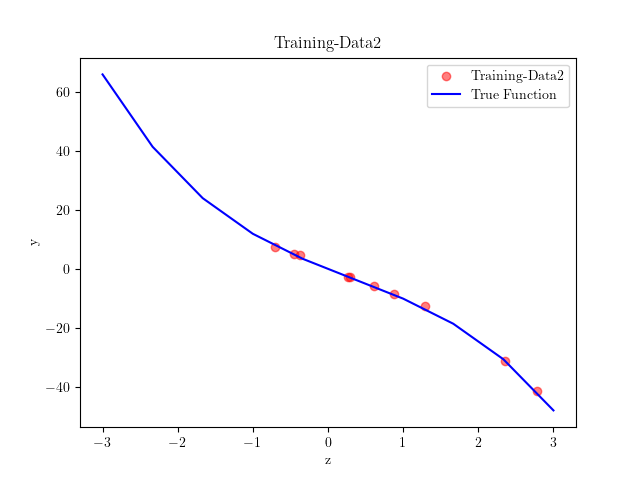
\includegraphics[width=0.8\textwidth]{../Graph/Training-Data2.png}
		      \caption{Training Data vs True Polynomial}
		      \label{fig:question9c}
	      \end{figure}

	      As it can be seen from the Figure \ref{fig:question9c} that the due to small sample size of the training data, it does not cover the whole polynomial function. This is the reason why the model is not able to learn the coefficients well.


	\item The value for a which should be selected is option A being the value 0.01. This is because if we select the option B in which the value of a is 5, then the function draws a polynomial line which is very tough to be learned with linear regression. In the other hand with option A since the range is very small, the polynomial line becomes linear and hence it is very easy to be learned with linear regression.

	      \begin{figure}[H]
		      \centering
		      \subfloat[Case A]{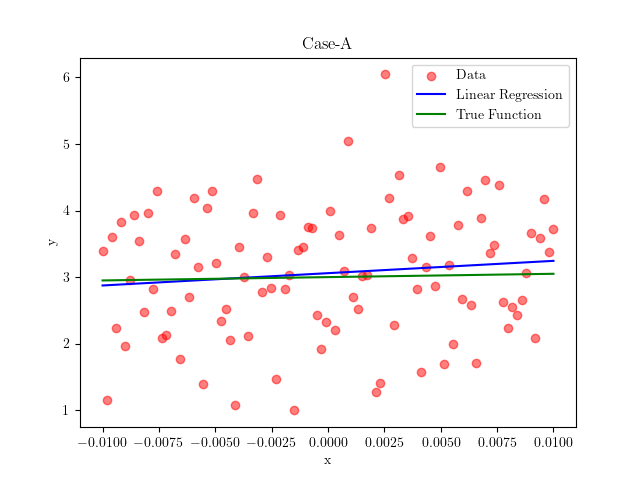
\includegraphics[width=0.45\textwidth]{../Graph/Case-A.png}\label{fig:question10a}}
		      \hfill
		      \subfloat[Case B]{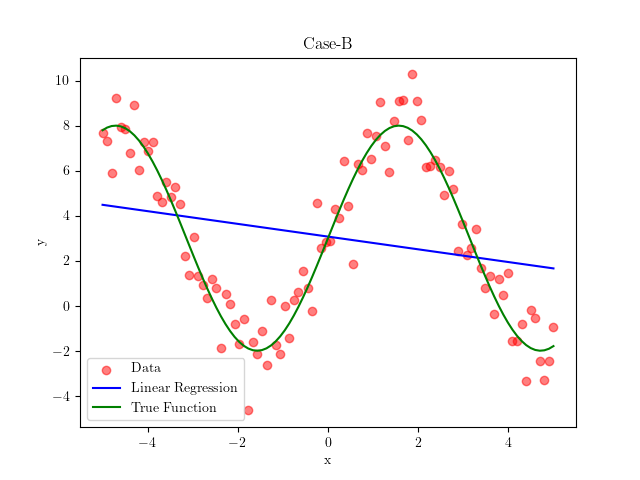
\includegraphics[width=0.45\textwidth]{../Graph/Case-B.png}\label{fig:question10b}}
		      \caption{Comparison of Case A and Case B} 
		      \label{fig:question10}
	      \end{figure}
	      As it can be seen from the Figure \ref{fig:question10} that the Case A is very easy to be learned with linear regression, but in the other hand Case B is very hard to be learned with linear regression. This is because in Case A the polynomial line is linear, but in Case B the polynomial line is not linear and hence it is very hard to be learned with linear regression.


\end{enumerate}


\section*{Questions}
\begin{enumerate}[(a)]
	\item No we do not need to chose different values of alpha. In Linear Regression it is common to use the same learning rate for the parameters. Usually you would want to use different learning rates if if you want to find a complex Global Minimum, but in this case of our Linear Regression we have only 2 parameters which does not require us to use different learning rates.
	\item The main principle behind choosing two different learning rates is to find a complex Global Minimum. In such cases there tends to be many local minimums which with a single learning rate is very is to converge to. Hence in such cases we should use different learning rates to find the complex Global Minimum. AdaGrad is such algorithm which follows the same principle, in which it uses different learning rates for different parameters. The learning rate for each parameter is inversely proportional to the sum of the squares of the gradients. Hence if the gradient is very large then the learning rate will be very small and if the gradient is very small then the learning rate will be very large. This helps in finding the complex Global Minimum.
\end{enumerate} 


\end{document}